\section{Linear Reward Inaction}
\subsection{Principe}
\begin{frame}{Principe}
\begin{itemize}
    \item Repose sur un \textbf{principe de récompense} lors d'une action positive.
    \item \textbf{Ne prends en compte ni la perte ni l'égalité}.\\~\
    \item On a un \textbf{vecteur stochastique de stratégie} pour chaque carte et joueur qui \textbf{se met à jour uniquement lors d'un gain}.
    \item Permet de trouver un \textbf{équilibre de Nash (en stratégies pures)} pour un.
\end{itemize}
\end{frame}

\begin{frame}{Algorithme de LRI}
\begin{figure}
    \centering
    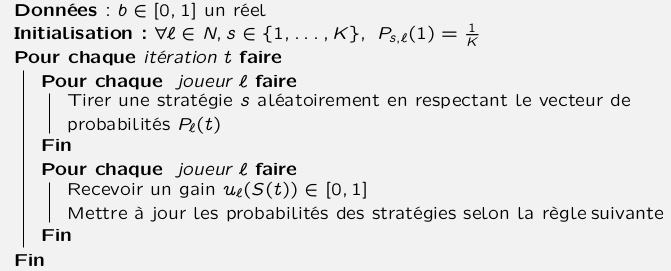
\includegraphics[width=\textwidth]{Images/algo/13.png}
    \label{fig:my_label}
\end{figure}
\centering K : nombre de stratégies.


%\begin{block}{Convergence de LRI [Sastry et Al. 1994]}
%\centering
%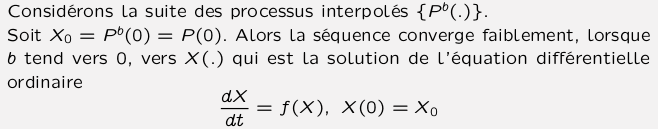
\includegraphics[width=0.60
%\textwidth,height=0.18\textheight]{Images/algo/14.png}
%\end{block}
\end{frame}

%%%%%%%
\begin{frame}{Mise à jour des stratégies des joueurs}
    \begin{block}{Règle de Mise à jour}
    $q_{i,s}(t+1)= \left\{\begin{array}{ll}
        q_{i,s}(t) + b * U_{t} * (1 - q_{i,s}(t))& \mbox{Si } s = s_i(t) \\
         q_{i,s}(t) - b * U_{t} * q_{i,s}(t) & \mbox{Si } s \neq s_i(t)
    \end{array}
\right.$
    \end{block}
    \begin{exampleblock}{Variables et constantes}
    \begin{description}
    \item[b] : paramètre d'apprentissage tq $b \in [0,1]$ et $b\leq \frac{1}{U_{max}}$.
    \item[$q_{i,s}(t)$] : probabilité que le joueur i joue la stratégie s à l'étape t.
    \item[$U_t$] : fonction d'utilité. %$U_t = \frac{Gain}{GainMax} =  \frac{Gain}{5}$
    \end{description}
    \end{exampleblock}
\end{frame}

%\begin{frame}{Propriété de la dynamique de LRI (Folk Theorem)}
%\begin{itemize}
%    \item Tous les équilibres de Nash sont des points stationnaires.
%    \item Tous les équilibres de Nash strict (en
%stratégies pures) sont asymptotiquement stables.
%    \item Tous les points stationnaires qui ne sont pas des Nash purs ne sont pas stables.
%\end{itemize}
%\end{frame}

\subsection{Application}

\begin{frame}{Étude de courbes}
\begin{columns}
        \begin{column}{0.5 \textwidth}
        \begin{small}
       \hspace{-0.24 cm} Probabilité qu'\textcolor{red}{Alice} se couche \\ Probabilité que \textcolor{blue}{Bob} se couche\\
        \end{small}
        \centering
            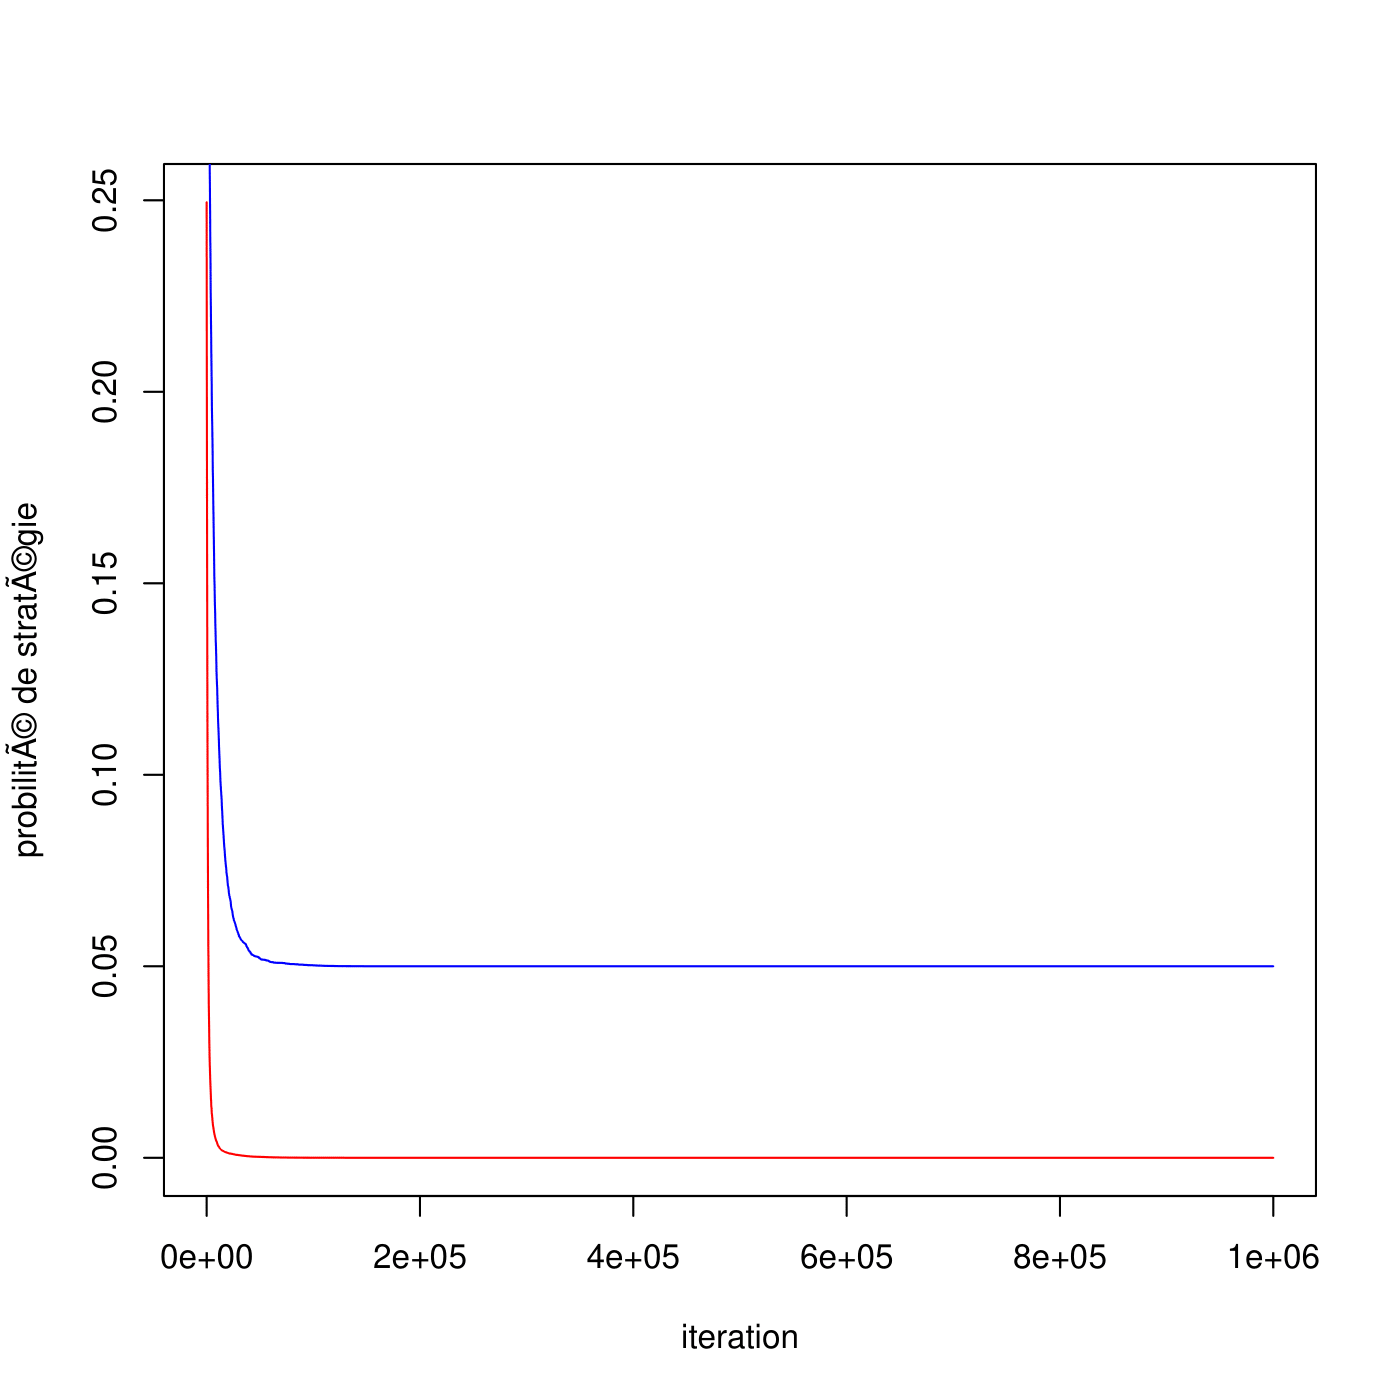
\includegraphics[width =\textwidth]{Images/Courbes/LRI/SeCoucher.png}
       
    
        \end{column}
       
        \begin{column}{0.5 \textwidth}
         \begin{small}
         \hspace{-0.24 cm} Probabilité qu'\textcolor{red}{Alice} relance de 4\\ Probabilité que \textcolor{blue}{Bob} suive\\
          \end{small}
        \centering
            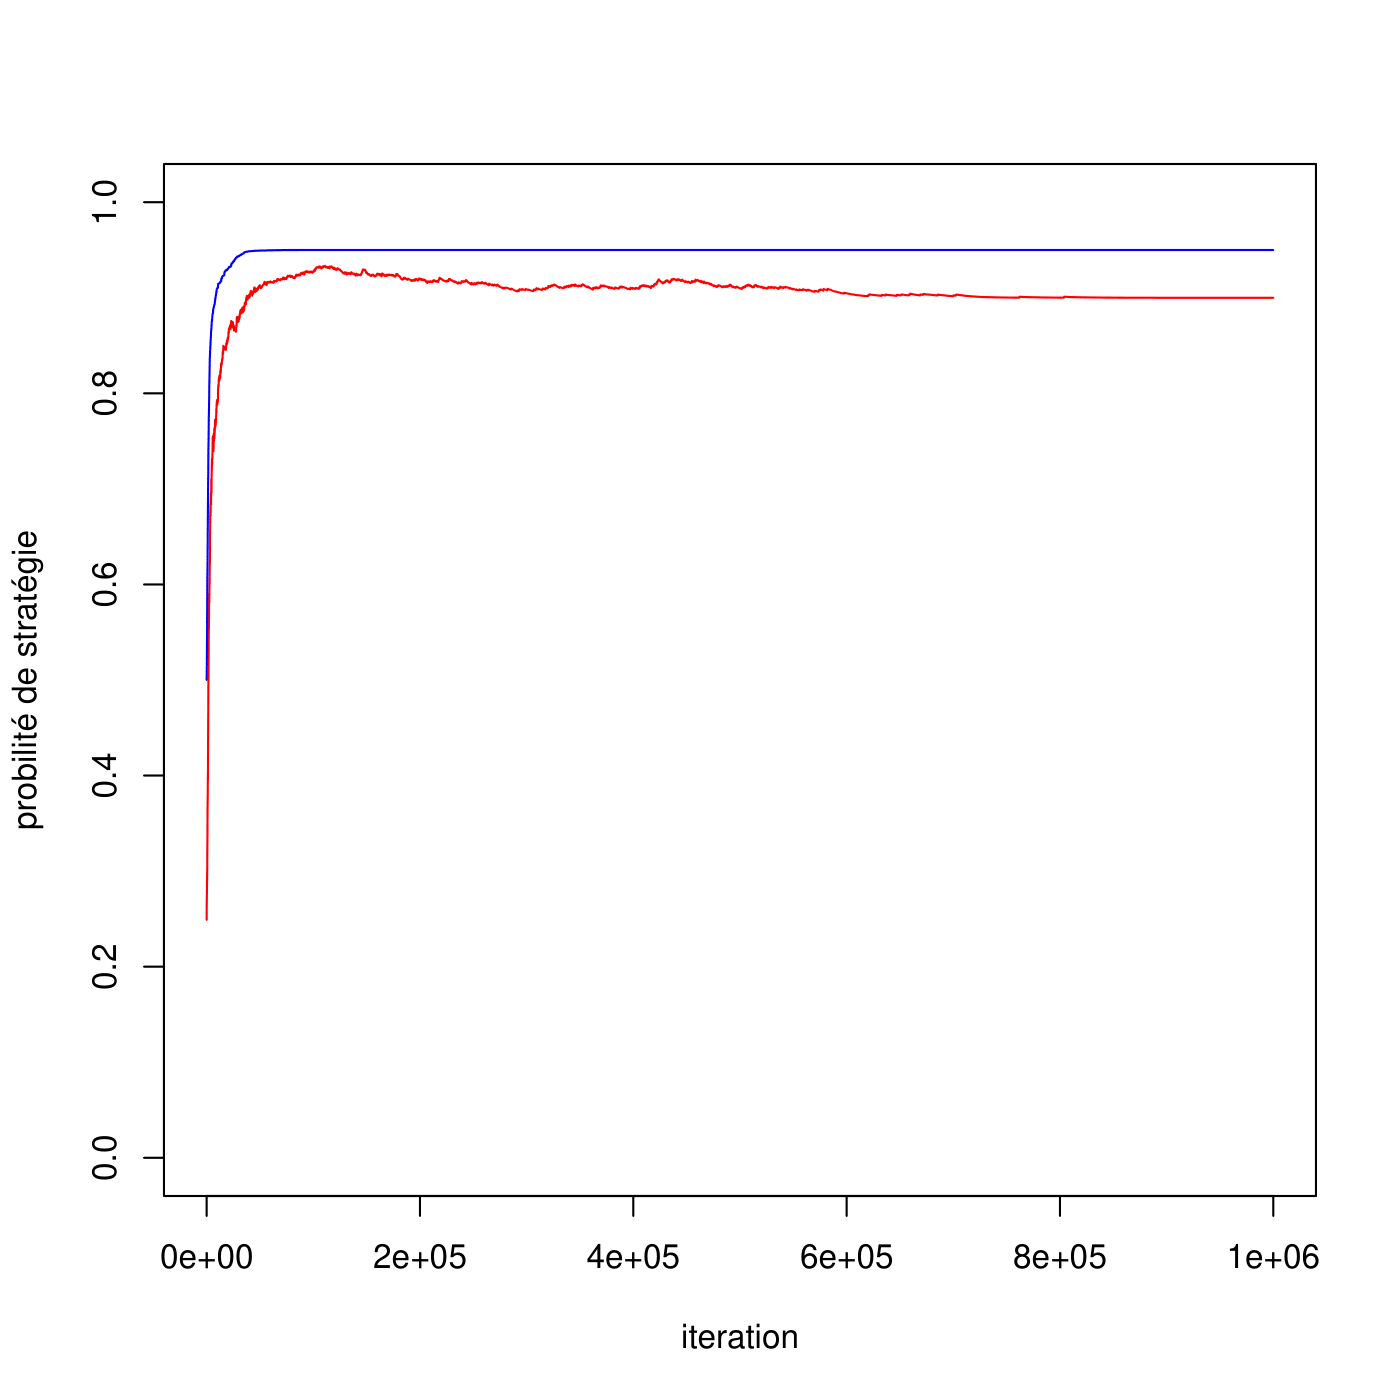
\includegraphics[width =\textwidth]{Images/Courbes/LRI/Relance4.png}
       
    \end{column}
    \end{columns}
\end{frame}

\begin{frame}{Étude de courbes}
\begin{columns}
        \begin{column}{0.5 \textwidth}
        \begin{small}
        \hspace{-0.24 cm} Probabilité qu'\textcolor{red}{Alice} relance de 1 \\ Probabilité que \textcolor{blue}{Bob} suive\\
        \end{small}
        \centering
            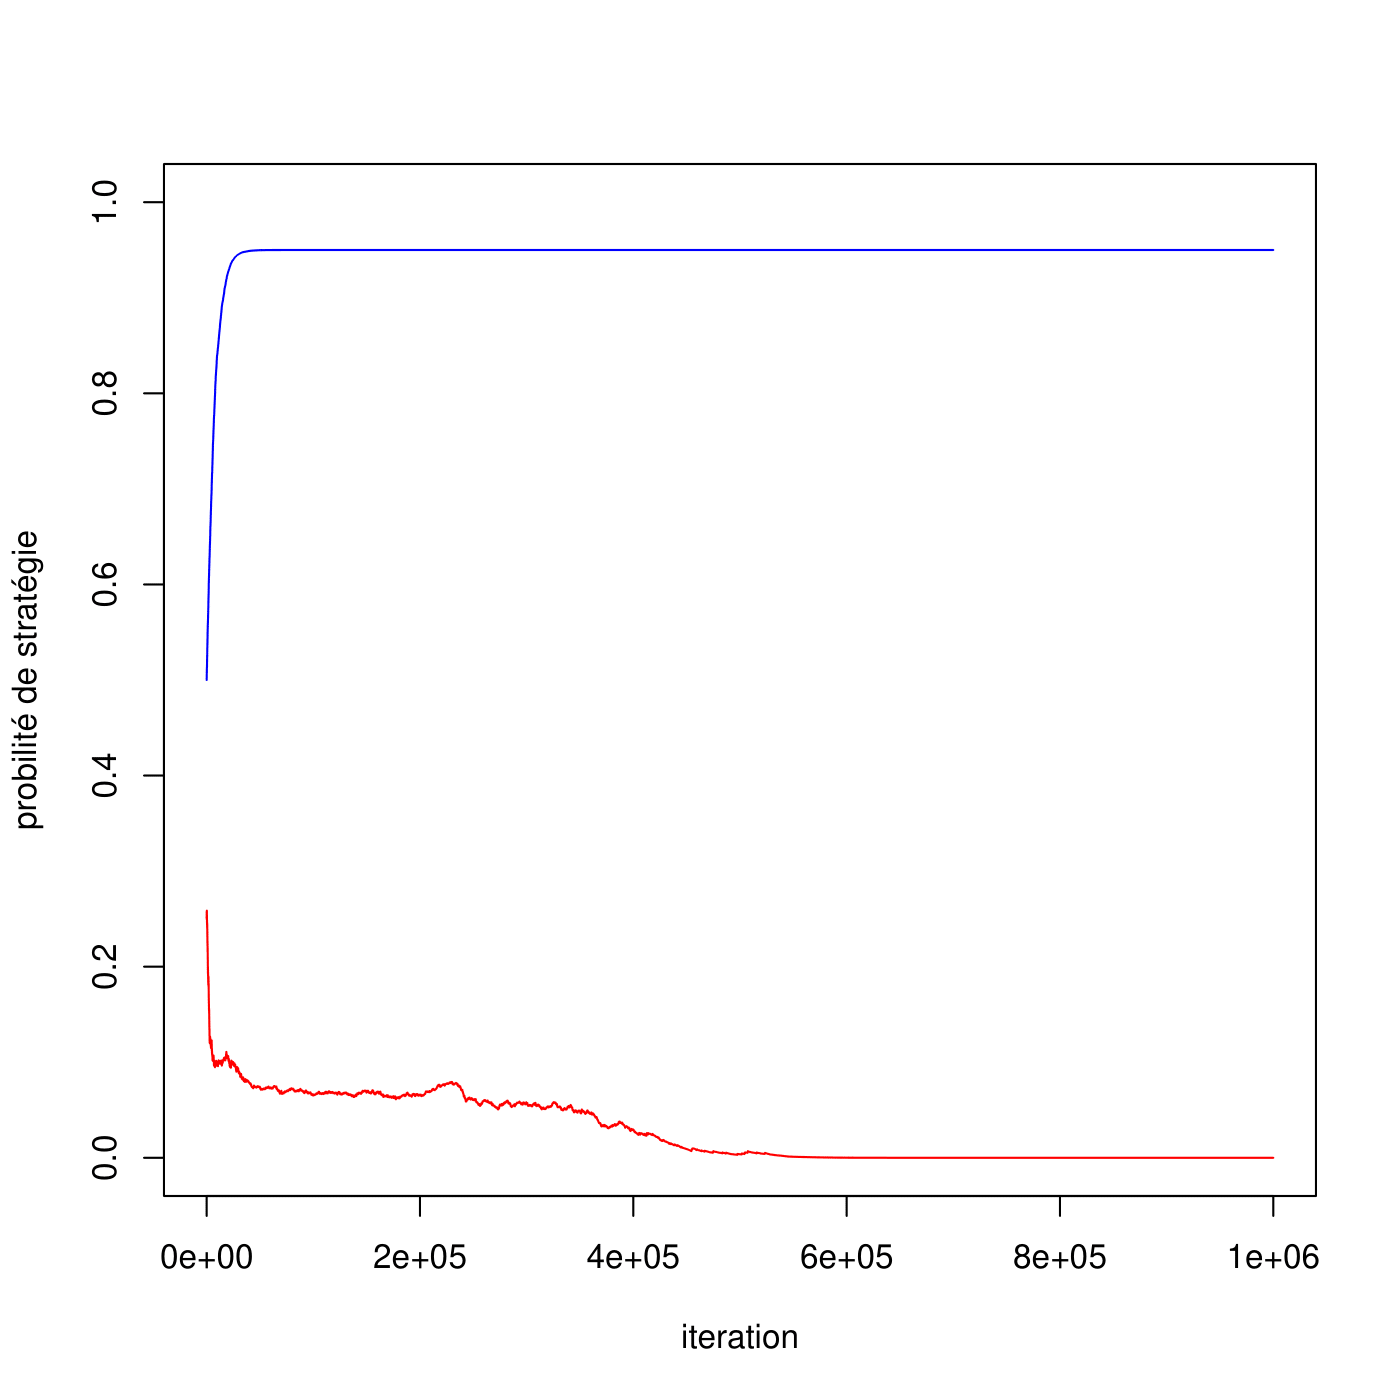
\includegraphics[width =\textwidth]{Images/Courbes/LRI/Relance1.png}
       
    
        \end{column}
       
        \begin{column}{0.5 \textwidth}
         \begin{small}
          \hspace{-0.24 cm} Probabilité qu'\textcolor{red}{Alice} relance de 2\\ Probabilité que \textcolor{blue}{Bob} suive\\
          \end{small}
        \centering
            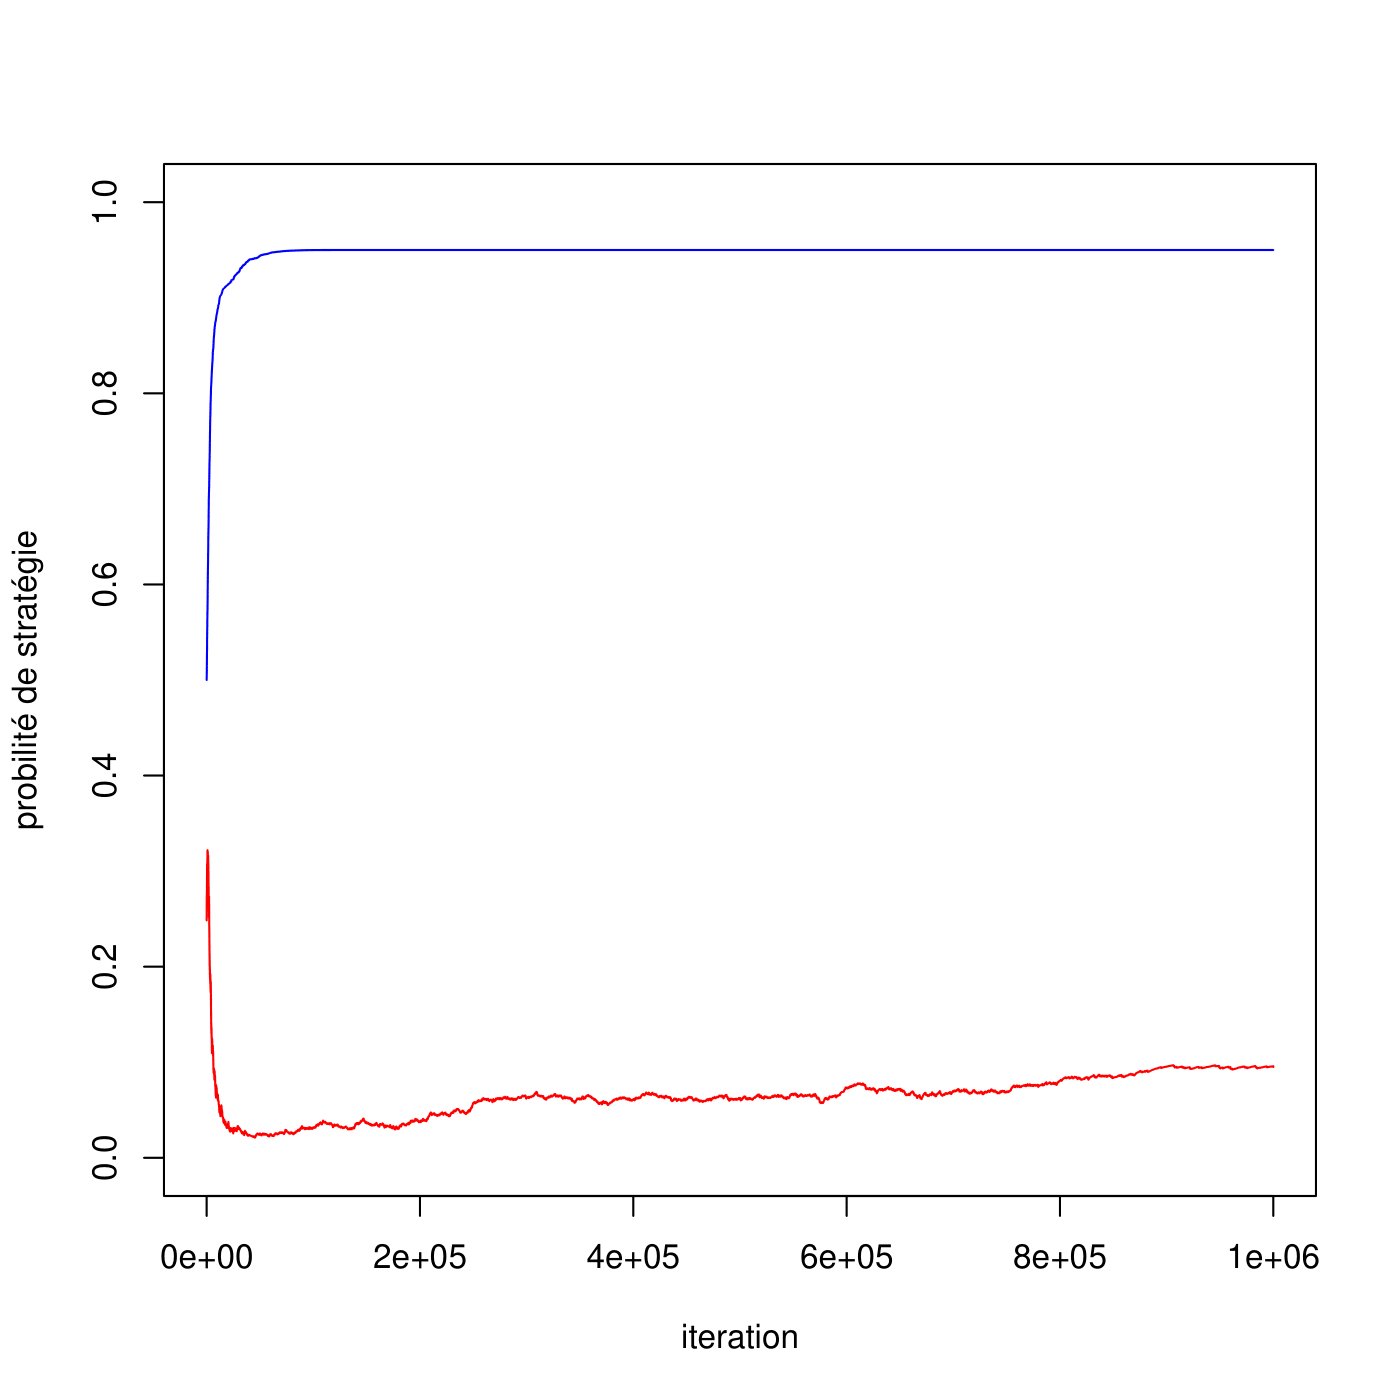
\includegraphics[width =\textwidth]{Images/Courbes/LRI/Relance2.png}
       
    \end{column}
    \end{columns}
\end{frame}

\begin{frame}{Étude de courbes}
Courbes des gains de \textcolor{blue}{Bob} et d\textcolor{red}{Alice} .
\centering
    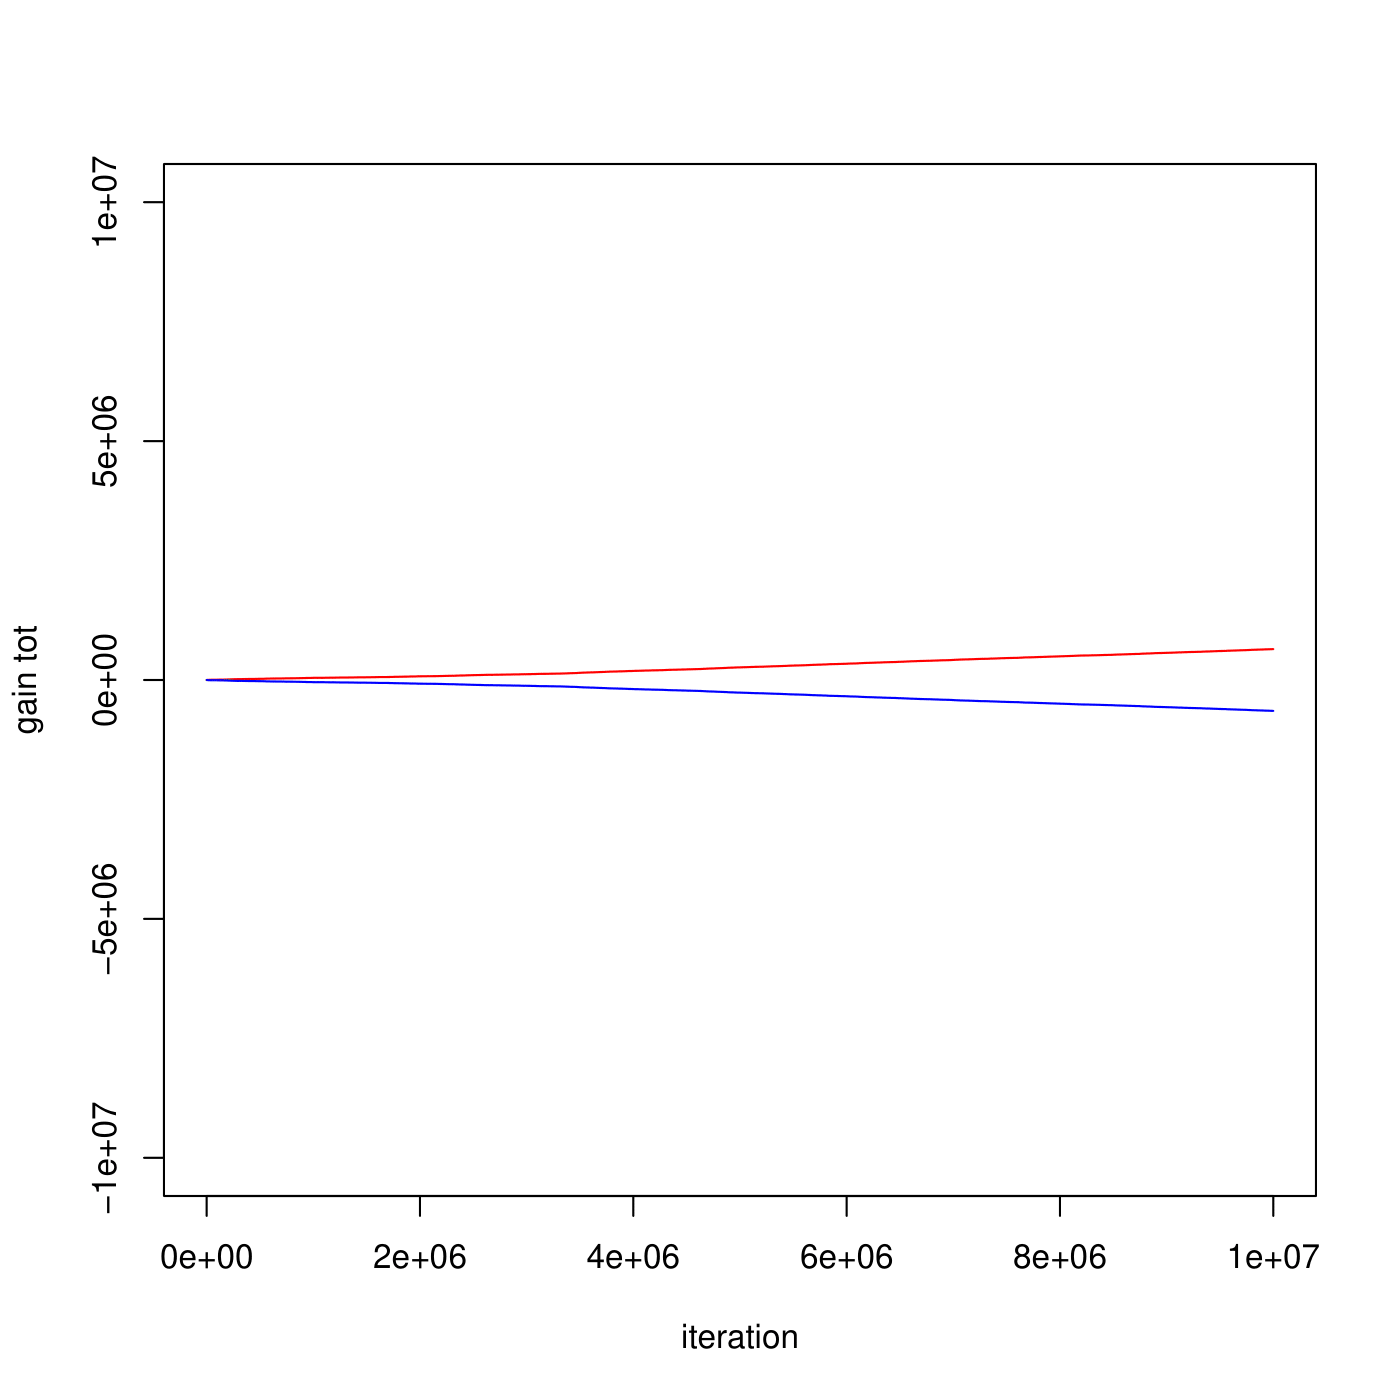
\includegraphics[width =1 \textwidth, height = 0.8 \textheight]{Images/Courbes/LRI/Gain.png}
\end{frame}

